\subsection{Mathematics Excursion I: Calculus}
Before we dive head-first into mechanics, we have to establish our ground rules. Over the course of this handout, we will be using calculus extensively/pretty much everywhere. Some of the prouder physicists would say calculus was invented to deal with mechanics in the first place! In this vein, it's important that we at least have some understanding of what calculus is and how to use it. 

It's okay if this section doesn't make complete sense if you haven't taken a calculus course -- this section is mostly intended to highlight a few important concepts, and as a reference as you proceed through the rest of the handout. You will definitely want to consult other texts to learn and practice calculus more extensively -- TJHSST uses \textit{Early Transcendentals} by Anton, Bivens, and Davis, of which copies can certainly be found online, although we do not condone or encourage the use of piracy to obtain educational materials. 

There are two main parts of single-variable calculus -- differential calculus (dealing with derivatives) and integral calculus (dealing with integrals). We'll look at these two as well as some of the more common applications of calculus to solve problems.
\subsubsection{Derivatives}
Derivatives describe how a function is changing over time. We may as well call it the "slope" of the function - ie. how much a function's output changes with respect to the input. For a function $f$ that is a line, the derivative of the function really is just the slope of the line, because remember that the slope for a line $y = mx+b$ is:
\[
	f'(x) = \dv{f}{x} = \dv{}{x}f(x) = m = \frac{\Delta y}{\Delta x} 
\]	
which is exactly the ratio of the change in the output to the change in the input.\\
The first three expressions are basically equivalent ways to write "the derivative of the function $f$ with respect to $x$." Whatever you want to use is up to you to denote the derivative, but I tend to use different notations depending on the situation. 
\begin{center}
	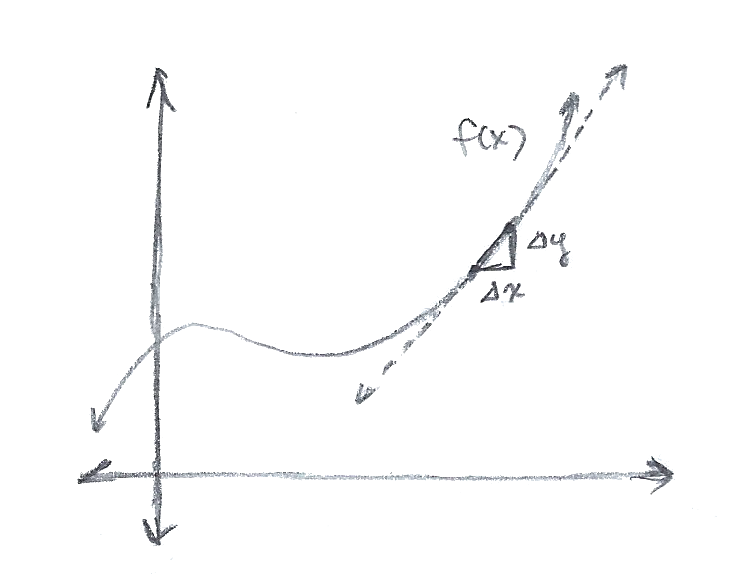
\includegraphics[scale=0.3]{images/math/calc/derivative.png}
\end{center}
What about for non-linear functions? We can still look at how a function's $y$-value changes due to small changes in $x$. If the change in $x$ is small enough, the region of the function around any $x$-value looks kind of like a line anyways. We can find an approximate value for the derivative of a function by looking at the value of the function on the interval $[x, x+h]$, where $h$ is some small real number: 
\[
	\dv{f}{x} \approx \frac{f(x+h) - f(x)}{x+h - x} = \frac{f(x+h) - f(x)}{h}
\]
To get the derivative of $f$, we let the value of $h$ go to zero, to see how the function changes instantaneously. Of course, we can't let $h$ equal zero, because that would be dividing by zero - but we can look at how this expression behaves for values of $h$ close to zero. This is the idea behind taking a limit, which in general allow you to look at what functions do as they approach certain values of $x$ (which you should have learned in TJ Math 5). 
\[
	\dv{f}{x} = \lim_{h\to 0} \frac{f(x+h) - f(x)}{h}
\]
This is the definition of the derivative of $f$ with respect to $x$. With this limit definition, we can start to compute the derivative for more complex functions. Let's look at the derivative of $f(x) = x^2$:
\[
	\dv{f}{x} = \lim_{h\to 0} \frac{f(x+h) - f(x)}{h} =  \lim_{h\to 0} \frac{(x+h)^2 - x^2}{h} =  \lim_{h\to 0} \frac{x^2 + 2xh + h^2 - x^2}{h} = \lim_{h\to 0} \frac{2xh + h^2}{h} = \lim_{h\to 0} 2x+h = 2x
\]
In general, it can be proven that if $f(x) = x^n$, for any real value of $n$: 
\[
	\dv{f}{x} = nx^{n-1}
\]	
This is called the power rule for derivatives. If $n$ is an integer, you can use the binomial theorem - but I'll leave that proof for you to discover. \\
Derivatives also satisfy the following properties, provable from the definition of the derivative:
The derivative of a sum or a multiple of two functions is the same as the sum or a multiple of the derivative of the functions. (This property is called linearity.) 
\[
	\dv{}{x}(f(x) + g(x)) = f'(x) + g'(x) \quad \dv{}{x}(cf(x)) = cf'(x) 
\]
For constant functions $f(x) = c$, we can see that 
\[
	\dv{f}{x} = \dv{}{x} (c) = 0
\]
For the product of functions, we can invoke the product rule, which states that:
\[
	\dv{}{x}(f(x) \cdot g(x)) = f'(x) g(x) + f(x) g'(x)
\]
Closely related is the quotient rule, which is applied for the quotient of two functions:
\[
	\dv{}{x}\left(\frac{f(x)}{g(x)}\right) = \frac{f'(x) g(x) - f(x) g'(x)}{g(x)^2}
\]
Most important of all is the chain rule for the composition of two functions $f(x)$ and $g(x)$:
\[
	\dv{}{x}f(g(x)) = \dv{f}{g} \cdot \dv{g}{x}
\]
What we mean by this notation is that wherever $g(x)$ is substituted in place of $x$ in $f(x)$, we take the derivative of $f(x)$ as if $g(x)$ were the variable, and then multiply by the derivative of $g(x)$ with respect to $x$. It would probably be more clear if I showed you a basic example - Let's look at the derivative of $f(x) = (3x+2)^2$. Let's evaluate this by expanding and taking the derivative of each term:
\[
	\dv{f}{x} = \dv{}{x} (9x^2 + 12x + 4) = 18x + 12
\]
Let's do this using the chain rule, assuming we're looking at the composition of the functions $x^2$ and $3x+2$:
\[
	\dv{f}{x} = 2(3x+2)^{1} \cdot 3 = 18x + 12
\]
The proof of the chain rule is the most complicated, and you can find proofs of all of these facts online. Using the limit definition, we can derive the derivatives of trigonometric, exponential, and logarithmic functions. I've listed them all here in a table:
\begin{center}
	\begin{tabular}{cc|cc|cc}
		\multicolumn{2}{c}{Trigonometric}&\multicolumn{2}{c}{Exponential}&\multicolumn{2}{c}{Inverse Trig}\\ \hline \hline \noalign{\smallskip}
		Function & Derivative & Function & Derivative & Function & Derivative \\ \hline \noalign{\smallskip}
		$\sin x$ & $\cos x$ & $e^x$ & $e^x$ & $\arcsin x$ & $\frac{1}{\sqrt{1-x^2}}$ \\ \hline \noalign{\smallskip}
		$\cos x$ & $-\sin x$ & $\ln x$ & $\frac{1}{x}$ & $\arccos x$ & $-\frac{1}{\sqrt{1-x^2}}$\\ \hline \noalign{\smallskip}
		$\tan x$ & $\sec^2 x$ & $a^x$ & $a^x \ln a$ & $\arctan x$ & $\frac{1}{1+x^2}$\\ \hline \noalign{\smallskip}
		$\cot x$ & $-\csc^2 x$ & $\log_a x$ & $\frac{1}{x \ln a}$ & $\arccot x$ & $-\frac{1}{1+x^2}$ \\ \hline \noalign{\smallskip}
		$\sec x$ & $\sec x \tan x$ & $c^f$ & $c^f \ln c\cdot f'$ & $\arcsec x$ & $\frac{1}{|x|\sqrt{x^2-1}}$ \\ \hline \noalign{\smallskip}
		$\csc x$ & $-\csc x \cot x$ & $f^{g}$ & $f^g \left(f'\frac{g}{f} + g' \ln f \right)$ & $\arccsc x$ & $-\frac{1}{|x|\sqrt{x^2-1}}$ \\ \hline \noalign{\smallskip}
	\end{tabular}
\end{center}
(The function $f(x) = e^x$ is defined so that its derivative is itself. The derivatives of other exponential functions are derived from the chain rule.) Using these principles, we can take the derivative of any elementary function and find out what it's rate of change using these rules.\\
We can also keep taking the derivative of the function as many times as we want, as long as the function is differentiable (meaning that the function is continuous and the limit involved in the derivative exists). We've only looked at the first derivatives of functions so far, but we can always find the second derivatives, third derivatives, etc. of functions. Notation-wise, we use $\dnv{y}{x}{n}$ for the $n$th derivative of a function, or $f^{n}(x)$ where $n$ is either expressed in Roman numerals if $n < 4$ or just written out regularly (which is in my opinion super arbitrary). Usually, however, we rarely go beyond the second derivative in physics. 

\subsubsection{Indefinite Integrals}
Given a function $f(x)$, let's try to find the function $F(x)$ that has $f(x)$ as its derivative. $F(x)$ is called the antiderivative of $f(x)$. We write $F(x)$ as the following:
\[
	F(x) = \int f(x) \, dx 
\]
The $dx$ at the end means that the antiderivative is being found with respect to the variable $x$. The big $\int$ symbol is called an integral, and finding the antiderivative is called taking the indefinite integral (or the integral, for short) - which is what I'll call it from now on, to avoid typing so much. \\
In general, it's much more difficult to integrate functions, and most of the time, the integral of a random composition of functions cannot be expressed as a combination of elementary functions. Let's just look at a simple example to start - the integral of $f(x) = x^2$. We can use a little bit of trial and error to do this. Notice that because of the power rule for derivatives, the exponents in polynomial functions decrease by 1. Therefore, we know that the antiderivative $F(x)$ has to be of the form $F(x) = kx^3$. By definition, 
\[
	\dv{}{x} F(x) = \dv{}{x} \int f(x) \, dx = f(x) 
\]
We know that $\dv{}{x} F(x) = 3 kx^2 = f(x)$. Therefore, $k = \frac{1}{3}$, so at the end of it all, we have:
\[
	F(x) = \int x^2 \, dx  = \frac{1}{3}x^3 + C
\]
Why add the $+C$? Because the derivative of a function eliminates the constant (the derivative of a constant is zero), any constant could have been added to the original function $F(x)$ to produce a derivative of $f(x)$. We can add any constant we want, but if we want to be as general as possible, we use a $+C$ represents any real number.\\
We don't have as many properties that hold in general for the evaluations of all integrals, but at least the properties of linearity still hold. That is, for any two functions, the integral of the sum or constant multiple of these functions is the sum or the constant multiple of the integral of the function:
\[
	\int f(x) + g(x) \, dx = \int f(x) \, dx + \int g(x) \, dx \quad \int cf(x) \, dx = c \int f(x) \, dx
\]
Here's a table of the most common integrals so you can get started: 
\begin{center}
	\begin{tabular}{c c}
		\multicolumn{2}{c}{Most Common Integrals}\\ \hline \noalign{\smallskip}
		Function & Antiderivative \\ \hline \hline \noalign{\smallskip}
		$\int x^n \, dx$ & $\frac{1}{n+1}x^{n+1}$ + C\\ \noalign{\smallskip} \hline \noalign{\smallskip}
		$\int e^x \, dx$ & $e^x + C$ \\ \noalign{\smallskip} \hline \noalign{\smallskip}
		$\int a^x \, dx$ & $\frac{1}{\ln a} a^x + C$ \\ \noalign{\smallskip} \hline \noalign{\smallskip}
		$\int \sin x \, dx$ & $-\cos x + C$ \\ \noalign{\smallskip} \hline \noalign{\smallskip}
		$\int \cos x \, dx$ & $\sin x + C$ \\ \noalign{\smallskip} \hline \noalign{\smallskip}
		$\int \sec^2 x \, dx$ & $\tan x + C$ \\ \noalign{\smallskip} \hline \noalign{\smallskip}
		%$\int \sec x \tan x \, dx$ & $\sec x + C$ \\ \noalign{\smallskip} \hline \noalign{\smallskip}
		$\int \tan x \, dx$ & $\ln |\sec x| + C$ \\ \noalign{\smallskip} \hline \noalign{\smallskip}
		$\int \frac{1}{x}\, dx$ & $\ln |x| + C$ \\ \noalign{\smallskip} \hline \noalign{\smallskip}
		$\int \frac{1}{\sqrt{1-x^2}} \, dx$ & $\arcsin x + C$ \\ \noalign{\smallskip} \hline \noalign{\smallskip}
		$\int \frac{1}{1+x^2}\, dx$ & $\arctan x + C$ \\ \noalign{\smallskip} \hline \noalign{\smallskip}
	\end{tabular}
\end{center}	
We do have some other tricks that we can use to evaluate more complex integrals. The most powerful is called the $u$-substitution, and it changes the variables inside the integral. Essentially, it's like the reverse of the chain rule, and works for integration. Let's just look at an example -  the integral $\int xe^{x^2} \, dx$. At first, this may seem really hard to do - after all, we don't know a function that has this as a derivative from the table, but what we can do is substitute $u = x^2$. When we do this, however, we also have to substitute in a new variable of integration (also called a differential) $du = 2x \, dx$. This is computed by taking the derivative of the substituted expression - note that $\dv{u}{x} = 2x$, so we just "multiply through" by $dx$. We substitute in $\frac{1}{2} u = x\, dx$ so we get:
\[
	\int xe^{x^2} \, dx = \int \frac{1}{2} e^u \, du = \frac{1}{2} e^u + C
\]
We can't leave our answer in terms of $u$, so we substitute back in to get: 
\[
	\int xe^{x^2} \, dx = \frac{1}{2}e^{x^2} + C
\]
Selecting the proper $u$-substitution for an integral can make the difference between making your job difficult and making your job easy. It takes a lot of practice to find the right $u$-substitution to simplify the integral to one of the most common integrals. \\
Another effective tool for evaluating integrals that involve products of functions. For functions $u$ and $v$ with differentials $du$ and $dv$, we have that:
\[
	\int u\, dv = uv - \int v \, du
\]
This is called the technique of integration by parts. For products of functions, even if the integral $\int u\, dv$ is hard to evaluate, we can transform it such that the new integral $\int v \, du$ is easier to evaluate. Let's look at the integral $\int x \sin x \, dx$. This is really hard to integrate on its own, but we can consider the products of the functions $u(x) = x$ and $v = -\cos x$. The differentials of these functions are $du = dx$ and $dv = \sin x \, dx$. If we plug this into the integration by parts formula, we have: 
\[
	\int x \sin x \, dx = -x \cos x - \int (- \cos x) \, dx = -x \cos x + \int \cos x \, dx
\]
We can evaluate the right side of the equation a bit more easily:
\[
	- x \cos x + \int \cos x \, dx = - x \cos x + \sin x + C
\]
Therefore, we have: 
\[
	\int x \sin x \, dx = -x \cos x + \sin x + C
\]
Our selection of $u$ and $v$ is a skill that can be improved with experience doing integrals. Usually, $u$ is a function that needs to be easily differentiated, and $dv$ needs to be easily integrated in order for the new integral to be easily evaluated. \\
A few other techniques that we will may look at throughout the course of the handout are using partial fractions to evaluate integrals and trigonometric substitution. We will address them as needed.

\subsubsection{Definite Integrals and the Fundamental Theorem of Calculus}
We can represent the accumulation of a quantity using a definite integral, and it has a close relation to the area that a function encloses. 
\begin{center}
	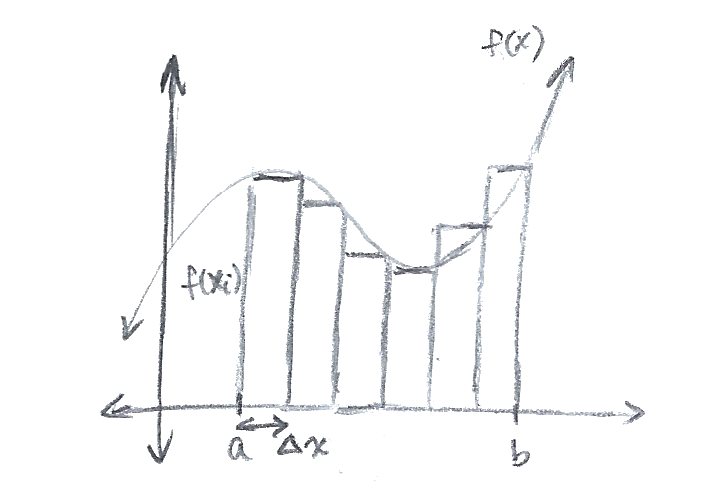
\includegraphics[scale=0.3]{images/math/calc/defintegral.png}
\end{center}
The area $A$ between the curve of $f(x)$ and $x-axis$ on the interval from $x = a$ to $x=b$ can be represented by a sum of many rectangles. If we subdivide the interval $[a,b]$ into $N$ equal intervals of length $\Delta x$, we can construct a rectangle in each interval that has width $\Delta x$ and height $f(x_i)$, where $x_i$ is the right-most $x$-coordinate of each interval. The area under the curve can be approximated by these rectangles. We can write this as:
\[
	A \approx \sum_{x_i \in [a,b]} f(x_i) \, \Delta x
\]
If we let the number of rectangles go to infinity and the width of each rectangle go to zero, we can approach the actual area of the curve. Therefore, we can write the area as a limit:
\[
	A = \lim_{N\to \infty , \Delta x \to 0} \sum_{x_i \in [a,b]} f(x_i) \, \Delta x = \int_a^b f(x) \, dx
\]
This is the definition of the definite integral, also called the Riemann integral. \\
We can also relate this to the indefinite integral. If $f(x)$ is the function that represents the rate of change of a function $F(x)$ with respect to $x$, every small rectangle in the area underneath the curve represents a small change in the value of $F(x)$. This is because that area represents the value of rate of change of $f(x)$ multiplied by the small change in $x$ ($dx$), which is the net change in $F(x)$, $\Delta F(x)$:
\[
	\Delta F(x) = f(x) \, dx
\]
If all of these small changes are summed up, the result is the net change in the function $F(x)$ on the interval $[a, b]$. Therefore, we can write the definite integral of a function $f(x)$ on the interval $[a, b]$ as the following:
\[
	\int_a^b f(x) \, dx = F(x)\Big|_a^b = F(b) - F(a) 
\] 
This is called the Fundamental Theorem of Calculus. We can now evaluate definite integrals by finding the antiderivative using an indefinite integral. This is incredibly useful for evaluating definite integrals, which we will do a lot during physics. 

\subsubsection{Differential Equations}
One of the applications for calculus is to create a model of a situation when the only information given is based on how things are changing at any particular point. Differential equations help us do this - they relate the derivatives of a function to the function itself. What if we want to do find a solution to a differential equation - that is, find an explicit expression for the function without involving its, given a few data points? This is extremely difficult in the general case, but in physics we will usually look at a few easier cases. \\
For the most part, we will be looking at first-order differential equations, where the only terms with derivatives involve the first derivative of the function. The most basic case is when the first derivative of a function only involves the independent variable $x$ (or $t$, $\theta$, etc.) and doesn't involve the function in the equation. For an example of this, let's look at the following function of $y$, assuming that we know that $y(0) = 1$:
\[
	\dv{y}{x} = e^{x} - 4x
\]
To solve it, we can just integrate with respect to $x$ from $0$ to some arbitrary real $r$: 
\[
	\int_0^r \dv{y}{x} \, dx = \int_0^r \, dy = \int_0^r e^{x} - 4x \, dx
\]
\[
	y(x)\Big|_0^r = (e^x - 2x^2)\Big|_0^r
\]
\[
	y(r) - y(0) = e^r - 2r^2 - 1
\]
\[
	y(r) = e^r - 2r^2 - 1 + y(0)
\]
Now, we see that the specific solution of the function that we're looking for depends on a data point. Since we know that $y(0) = 1$, we can simply plug in this value to get:
\[
	y(x) = e^x - 2x^2
\]
Since there's nothing special about our choice of $r$, it's simply standing in as a dummy variable - so I can replace it with $x$ or really anything I want. If I had changed the value of our initial data point, we could have had any arbitrary constant added onto the end of this, and it still would satisfy the original differential equation. In general, however, adding a constant to the end of any solution to a differential equation won't necessarily always allow it to satisfy the original equation. Let's look at another example: 
\[
	\dv{y}{x} = xy 
\]
In this case, we have the original function involved, so just integrating won't work. However, we can "separate" the variables by moving everything with a $y$ to one side and everything with an $x$ in it to another: 
\[
	\frac{1}{y} \, dy = x \, dx
\]
Now we can integrate with respect to each differential:
\[
	\ln |y| = \frac{1}{2}x^2 + C
\]
We can now solve for $y$:
\[
	y = e^{\frac{1}{2}x^2 + C} = Ce^{\frac{1}{2}x^2}
\]
Notice that because of the exponentiation, you can only manipulate the constant as a scale factor and not as an added constant. If you try substituting this back into the original equation, you can see that it works in general, whereas if you try adding a constant to the function instead it won't work. \\
In the text, I solve differential equations by moving all the terms to one side and integrating, which is essentially the same as separation of variables and results in the same solutions. Separation of variables is generally better for finding general solutions, but I use a shortcut for plugging in the data point to create the specific solution to match the situation. 

\subsubsection{Taylor Series Expansions}
The final tool that we use for solving problems are Taylor series. I claim that if a function is differentiable to an arbitrarily large degree at a point, I can approximate the behavior of the function as a polynomial at that point. (For simplicity, we'll assume that this point is at $x=0$.)\\
To create a polynomial that matches the behavior of the function at a point, all of the derivatives of the function at the point should match that of the polynomial. Let's be more specific - say the function is $f(x)$, and we know the values of $f(0), f'(0), f''(0),$ etc. We can try to build a function $p(x)$ that matches the $n$th-derivative at $x=0$. \\
If we just want to match $f(x)$ at $x=0$, we could just have $p(x) = f(0)$. This isn't a very good approximation of the function everywhere, though - it only matches the function at this point. Let's try again. \\
If we also want to make $p'(x)$ match $f'(x)$ at $x =0$, we could use a line - consider $p(x) = f(0) + f'(0) x$. Notice that this function has derivative $p(x) = f'(0)$, so it works. \\
Let's keep going to the second derivative. We want to add a term, but also make sure that the added term doesn't mess up what we had before. Because after taking two derivatives only polynomial terms of degree 2 will be constant, the added term should look like $kx^2$ for some $k$. If we take two derivatives of this term, the constant term that's left should look like $2k$ (because of the power rule). In order for us to have the right second derivative at $x = 0$, the coefficient $k = \frac{f''(0)}{2}$. So far, then, $p(x) = f(0) + f'(0)x + \frac{f''(0)}{2}x^2$ will match $f(x)$ for the first two derivatives and the value of $f(0)$. \\
We can continue on like this. The polynomial $p(x) = f(0) + f'(0)x + \frac{f''(0)}{2} x^2 + \frac{f'''(0)}{6} x^3$ will match $f(x)$ at the first three derivatives at $x=0$ (show this yourself) and we can keep adding on to infinity, basically. In general, we can make an infinite polynomial as follows that will be exactly $f(x)$:
\[
	f(x) = \sum_{i=0}^{\infty} \frac{f^{i}(0)}{i!}x^i
\]
This infinite polynomial is called the Taylor series of $f(x)$. A lot of the time, we will approximate functions using Taylor series if their inputs are close to zero. In these scenarios, we will basically just appproximate the first non-zero term to be the value of the function close to zero. Let's look at the function $\sin x$ (a function that we will approximate a lot) and compute the derivatives of $\sin x$ at $x=0$:
\[
	\sin (0) = 0
\]
\[
	\dv{}{x} \sin x = \cos x \rightarrow \dv{}{x} \sin x \Big|_{x=0} = \cos (0) = 1
\]
\[
	\ddv{}{x} \sin x = -\sin x \rightarrow \ddv{}{x} \sin x \Big|_{x=0} = -\sin (0) = 0
\]
\[
	\dnv{}{x}{3} \sin x = -\cos x \rightarrow \dnv{}{x}{3} \sin x \Big|_{x=0} = -\cos (0) = -1
\]
\[
	\dnv{}{x}{4} \sin x =  \sin x \rightarrow \dnv{}{x}{4} \sin x \Big|_{x=0} =  \sin (0) = 0
\]
Since the derivatives of $\sin x$ basically cycle through every four derivatives, we know that the Taylor series of $\sin x$ is:
\[
	\sin x = 0 + 1 \cdot x + \frac{0}{2} x^2 + \frac{-1}{6}x^3 + \frac{0}{24}x^4 + \ldots = \sum_{i = 0}^{\infty} \frac{(-1)^i}{(2i+1)!}x^{2i+1}
\]
The first non-zero term you see here is $x$, so we commonly approximate $\sin x = x$ for $x$ close to zero. (And now hopefully you understand math memes a little better.) \\
Taylor series are pretty important - although we don't use them in the text, some of the problems do require their use in order to solve them. 
\pagebreak